% Make nice A4 pages for print:
%\usepackage{pgfpages}
%\pgfpagesuselayout{resize to}[a4paper,border shrink=5mm,landscape]

\beamertemplatenavigationsymbolsempty

\setbeamertemplate{bibliography item}[text]

\usepackage[type={CC},modifier={by-sa},version={4.0}]{doclicense}

\usepackage[utf8]{inputenc}
\usepackage{hyperref}
\usepackage{breakurl}
\usepackage{graphicx}
\usepackage{pgfplots}
\usepackage{pgf}
\usepackage{tikz}
\usetikzlibrary{positioning}
\usetikzlibrary{arrows}
\usetikzlibrary{decorations.markings}
\usetikzlibrary{calc}
\usetikzlibrary{matrix}
\usetikzlibrary{shapes}
\usetikzlibrary{decorations.pathmorphing}
\usetikzlibrary{fit}
\usetikzlibrary{backgrounds}
\usetikzlibrary{plotmarks}
\usepackage{stmaryrd}
\usepackage{listings}
\usepackage{pdflscape}
\usepackage{perpage}
\usepackage{appendixnumberbeamer}

%\usepackage[thmmarks,amsmath,amsthm]{ntheorem} % already included in beamer
\usepackage{thm-restate}

\usepackage[sort&compress,numbers]{natbib}  % to be have \citet, \citeauthor, \citeyear

\MakePerPage{footnote}

\tikzstyle{o}=[r,ppBlue]
\tikzstyle{r}=[thick,rectangle,align=center]
\tikzstyle{t}=[r,ppTrans] %,font=\bfseries]
\tikzstyle{dd}=[densely dashed]
\tikzstyle{n}=[r,ppBlue]
\tikzstyle{p}=[r,ppRed]
\tikzstyle{ppRed}  =[draw=red,  fill=  red!20]
\tikzstyle{ppBlue} =[draw=blue, fill= blue!20]
\tikzstyle{ppGreen}=[draw=green,fill=green!20]
\tikzstyle{ppTrans}=[draw=none, fill=none]

\usetheme{Warsaw}

\useoutertheme[subsection=true]{smoothbars}
%\useoutertheme[subsection=false]{miniframes}

\definecolor{bblue}{HTML}{D7DF01}	% yellow-ish actually, for better black/white printing
\definecolor{rred}{HTML}{C0504D}
\definecolor{ggreen}{HTML}{9BBB59}
\definecolor{ppurple}{HTML}{9F4C7C}
\definecolor{lightgray}{rgb}{0.3,0.3,0.3}
\definecolor{lightergray}{rgb}{0.9,0.9,0.9}
\definecolor{UniBlue}{RGB}{83,121,170}

\DeclareTextFontCommand\textintro{\normalfont\bfseries\itshape} % nice!
\newcommand{\intro}[2][]
{%
	\textintro{#2}%
}
\newcommand{\empha}[2][]
{%
	\emph{#2}%
}

%\theoremstyle{plain}
\newcounter{reqcounter}
\newtheorem{requirement}[reqcounter]{Requirement}

%setbeamercolor{structure}{fg=violet}

\makeatletter
\def\th@task{%
    \normalfont % body font
    \setbeamercolor{block title example}{bg=orange,fg=white}
    \setbeamercolor{block body example}{bg=orange!20,fg=black}
    \def\inserttheoremblockenv{exampleblock}
  }
\makeatother

\theoremstyle{task}
\newtheorem{task}{Task}

\newenvironment{assignment}%
{%\setbeamercolor{background canvas}{bg=violet}%
%\setbeamercolor{structure}{fg=cyan!90!black}%
 \setbeamercolor{frametitle}{bg=orange,fg=white}
\begin{frame}}%
{\end{frame}}%

\AtBeginSection[]{
  \begin{frame}
  \vfill
  \centering
  \begin{beamercolorbox}[sep=8pt,center,shadow=true,rounded=true]{title}
    \usebeamerfont{title}\insertsectionhead\par%
  \end{beamercolorbox}
  \tableofcontents
  \vfill
  \end{frame}
}




\pgfplotsset{compat=1.14}
\author{Markus Raab}


\title{L02 Configuration Specification Languages}
\date{17.03.2021}

\begin{document}

%%%%%%%%%%%%%%%%%%%%%%%%%%%%%%%%%%%%%%%%%% 
\section{Theory}

\begin{frame}
	\frametitle{Rationale}
	\begin{itemize}
	\item without specification you and others do not even know which settings are available
	\item needed for any further techniques we will discuss
	\pause
	\item essential for \intro[no-futz computing]{no-futz computing}~\citet{holland2001nofutz}
	\item the foundation for any advanced tooling like configuration management tools
	\pause
	\item needed as communication of producers and consumers of configuration
	\end{itemize}
\end{frame}

\begin{frame}
	\methodQuestion{}
	\question{Configuration specification (e.g. XSD/JSON schemas) allows you to describe possible values and their meaning.  Why do/would you specify configuration?}
	\ExecuteMetaData[../book/motivation.tex]{question-introduce-spec}
\end{frame}

\begin{frame}
	\frametitle{Limitations of Schemata designed for Data}
	\begin{itemize}
	\item e.g.\ XSD/JSON schemas
	\item they are already very helpful but:
	\pause
	\begin{itemize}
	\item not key-value based
	\item not easy to introspect
	\item designed to validate data without semantics: \\ file path vs.\ presence of file
	\item not always possible to extend with plugins
	\item tied to specific formats (e.g. XML/JSON)
	\end{itemize}
	\end{itemize}
\end{frame}

\begin{frame}
	\frametitle{Types of Specifications}
	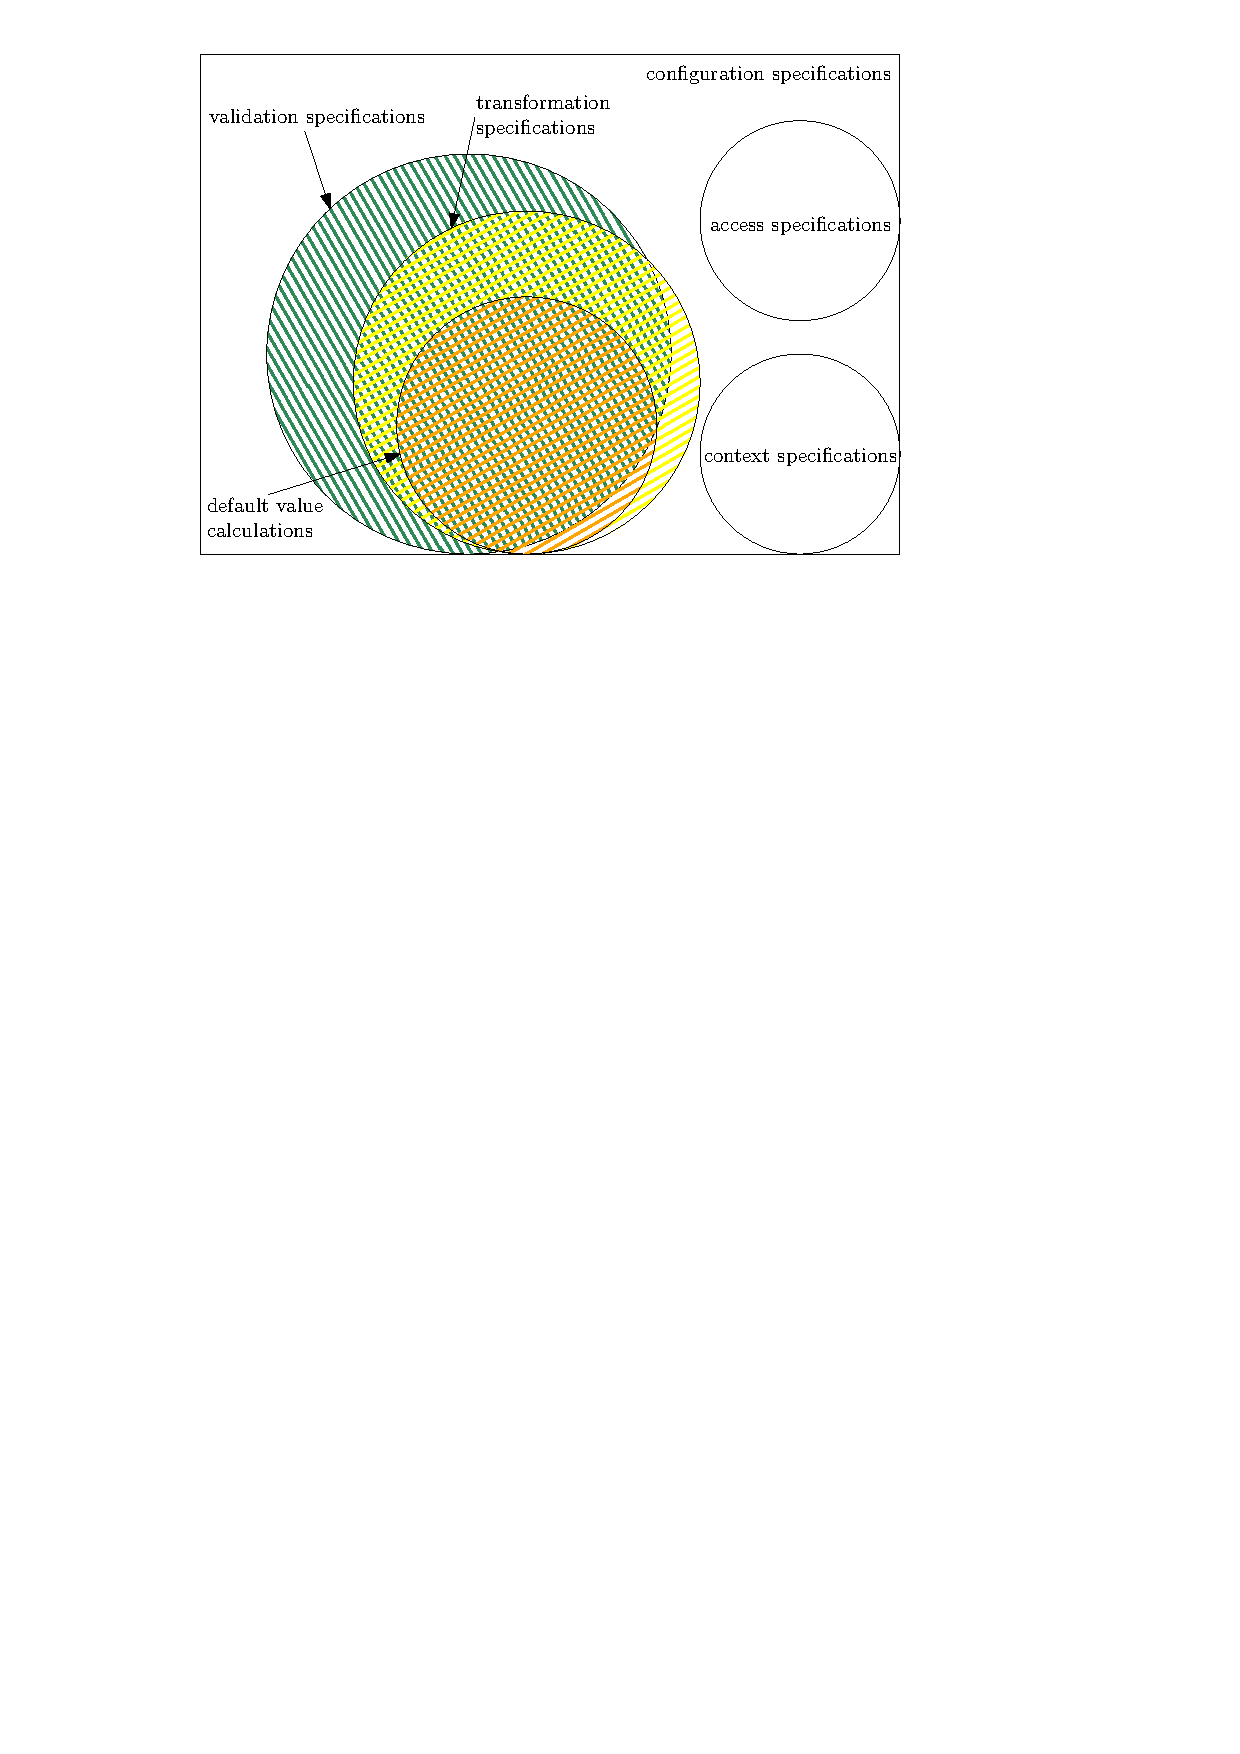
\includegraphics[scale=0.8]{specifications}
\end{frame}


\begin{frame}
	\frametitle{Requirements}

	\begin{itemize}
	\item formal/informal?
	\item complete?
	\pause
	\item should be extensible
	\item should be external to application
	\item open for introspection (for tooling)
	\item should talk to users
	\item should allow generation of artefacts
	\end{itemize}
\end{frame}


\begin{frame}[fragile]
	\frametitle{Grammar}
	\begin{grammar}
	<configuration specifications> ::= \{ <configuration specification> \}

	<configuration specification> ::= '[' <key> ']' <properties>

	<properties> ::= \{ <property> \}

	<property> ::= <property name> ':=' [ <property value> ]
	\end{grammar}

	\vspace{1cm}
	Example:
	\begin{code}[gobble=4]
	[slapd/threads/listener]
	default:=1
	type:=long
	\end{code}
\end{frame}


\section{Practise}

\begin{frame}[fragile]
	\frametitle{Options}

	Environment and command-line options can be considered with:

	\begin{code}[morekeywords={long,env},gobble=4]]
	[recursive]
	  type:=boolean
	  opt:=r
	  opt/long:=recursive
	  env:=RECURSIVE
	  default:=0
	\end{code}
\end{frame}

%TODO: currency

\begin{frame}[fragile]
	\frametitle{Examples}
	Sharing:
	\begin{code}[gobble=4]
	[slapd/threads/listener]
	fallback/#0:=slapd/threads
	\end{code}

	\vspace{1cm}
	Percentages
	\\ (e.g., configured image should be additionally cropped):
	\pause
	\begin{code}[gobble=4]
	[image/width]
	type:=long

	[crop]
	type:=long
	check/range:=0-100
	\end{code}
\end{frame}

\begin{frame}
	\frametitle{Visibility}
	\begin{itemize}
	\item idea: show only relevant settings for specific user group
	\item or disallow editing: accessibility
	\pause
	\item requires user-feedback loops~\cite{xu2015hey}
	\item most-used settings should be best visible (or even enforce them to be changed: against harmful defaults)
	\item think of your users (administrators), \\ only expose what users need
	\item write an rationale why someone needs it
	\pause
	\item visibility should not be an excuse to add not-needed settings
	\end{itemize}
\end{frame}

\begin{frame}[fragile]
	\frametitle{Example}
	\begin{code}[gobble=4]
	[slapd/threads/listener]
	visibility:=developer

	[slapd/access/#]
	visibility:=user
	\end{code}
\end{frame}


\begin{assignment}
	\begin{task}
	Brainstorming: Now, how do we implement such a specification?
	\end{task}
\end{assignment}

\begin{frame}
	\frametitle{Possible Implementations}
	\begin{itemize}
	\item tooling (GUI, Web UI)
	\item generate examples/documentation
	\item auto-completion/syntax highlighting/IDE support
	\item plugins in configuration framework (hide settings)
	\end{itemize}
\end{frame}




\section{Meeting}
%TODO: add cliffhanger with preview for next time

\begin{assignment}
	\begin{task}
	Brainstorming: What can be part of a configuration specification?
	What can they be used for?
	\end{task}
\end{assignment}

\begin{assignment}
	\begin{task}
	What do we mean with a configuration specification?
	\end{task}

	\begin{task}
	Which requirements do we have for a configuration specification?
	\end{task}
\end{assignment}

\begin{assignment}
	\begin{task}
	Break.
	\end{task}
\end{assignment}




%%%%%%%%%%%%%%%%%%%%%%%%%%%%%%%%%%%%%%%%%% 
\nocite{raab2017introducing}

\appendix

\begin{frame}[allowframebreaks]
	\bibliographystyle{plainnat}
	\bibliography{../shared/elektra.bib}
\end{frame}

\end{document}


